\chapter{Quizz 2}
On trouvera dans cette section le materiel qui est testé dans le quizz 2 qui est: 
\begin{itemize}
    \item Sets
    \item Functions
    \item Relations
    \item Sequences
\end{itemize}
\section{Set}

\begin{definition}[set]
    Une set est une collection d'objets sans ordre
\end{definition}
Par exemple:
\begin{itemize}
    \item Les étudiants en ba1 d'informatique
    \item les chaises dans une classe
\end{itemize}
Les objets d'une set sont appellés \textbf{elements} de la set. comme vu en analyse, la notation $a \in A$ nous informe que $a$ appartient à $A$ et inversement, $a \notin A$ insinue que $a$ n'est pas dans la set.
\\
Une set en AICC (et en informatique en général) est une analogie de l'ensemble en analyse (notion vu dans les premières semaine de cours). On a donc les même opération comme l'addition, soustraction, conjonction... 
\hspace{0.4cm}
\newpage

\begin{framedremark}
    Dans le cours d'AICC 1 pour les entiers positifs ($\mathbb{Z}^+$) et les réel positifs ($\mathbb{R}^+$), $0$ n'y est pas inclus.
\end{framedremark}

\subsection{Empty Set}
\begin{itemize}
    \item L'\textbf{empty set} et une set qui ne possède aucun élément.
    \item On l'appelle aussi \textbf{null set}
    \item Le symbole correspondant: $\emptyset$, où $\emptyset = \{\}$
\end{itemize}

Attention à ne pas confondre $\{\emptyset\}$ avec une empty set. $\{\emptyset\}$ est la set contenant l'empty set qui est équivalent à : $\{\{\}\}$.

\subsection{Subsets}
On peut voir les subsets comme des "\textit{Poupées russes}" de sets. Formellement : 
\begin{definition}[Subset]
    Une set $A$ est une subset de $B$, et $B$ est une superset de $A$ si et seulement si tout les éléments de $A$ sont aussi un élément de $B$.
\end{definition}
On peut le voir comme ça: 

\begin{center}
    
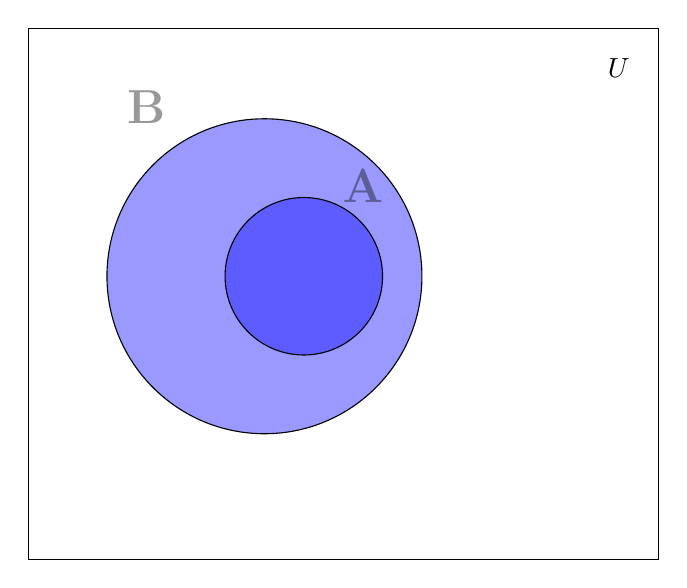
\begin{tikzpicture}

	\begin{scope} [fill opacity = .4]

    \draw[fill=blue, draw = black] (-1,0.85) circle (2);
    \draw[fill=blue, draw = black] (-0.5,0.85) circle (1);

    
    \node at (-2.5,3) {\LARGE\textbf{B}};
    \node at (0.25,2) {\LARGE\textbf{A}};
    \draw[](4, -2.75) rectangle (-4, 4);

    \end{scope}
    \node at (3.5, 3.5) {$U$};
    
\end{tikzpicture}
\end{center}

On voit ici $A$ une subset de $B$ se trouvant à l'intérieur de $B$. Attention, si A faisait la taille de B et recouvrait tout les éléments mais pas plus que $B$ alors elle serait aussi une subset de $B$. 
\begin{framedremark}
    A noter ici la set $U$ qui représente l'univers en sont entièreté. Il est utile lorsqu'on recherche à faire le complément d'une set.
\end{framedremark}

La notation, $A \subseteq B $ nous informe que $A$ est une subset de $B$
\\
Si $A \subseteq B$ mais que $A \neq B$ alors on dit que $A$ est une \textbf{proper subset} de $B$. Pour l'écrire en logique : 
\begin{equation*}
    \forall x (x\in A \implies x \in B) \wedge \exists x (x \in B \wedge x \notin A)
\end{equation*}
En français, cela veut dire, Tout éléments appartenant à $A$ appartiennent aussi à $B$ et il existe un élément tel qu'il appartient à $B$ mais pas à $A$.
\\
\\
On le note :
\begin{center}
 $A \subset B$.
\end{center}
\subsection{Power Set}
\begin{definition}[power set]
    Une set de toute les subsets de $A$, dénoté comme $\rho(A)$ ($\rho(A)$ est la fonction qui créer la subset) est appelée la \textbf{power set} de $A$.
\end{definition}
\hspace{0.4cm}
Par exemple si on prend $A = \{ a, b\}$ alors $\rho(A) = \{\emptyset, \{a\}, \{b\}, \{a, b\}\}$ est la power set de $A$. On remarque déjà plusieurs choses ici, 
\begin{itemize}
    \item $\emptyset$ fait toujours parti de la power set, $\emptyset$ est une subset de n'importe quel set (même elle-même).
    \item La set elle-même (donc $\{A\}$ Pour la set $\{A\}$) faire aussi toujours parti de la power set.
\end{itemize}
On voit donc que pour une set de taille $1$, alors la taille de la power set est de $2$. Si on prend maintenant une set de taille $n$, alors la power set est de taille : $2^n$.
\begin{framedremark}
    Il est possible et on verra plus tard de fabriquer une power set avec le diagram d'Hasse afin de mieux se la visualiser.
\end{framedremark}

\subsection{calcul sur des sets}
Comme dit auparavant, il existe des opérations sur les sets comme l'union ($A \bigcup B$), l'intersection ($A \bigcap B$) la Différence ($A - B$) le complément (comme en probabilité, $\overline{A}$ ou $A^\complement$).
\\
Voici avec un diagrame de Vienne deux set $A$ et $B$:
\begin{center}
    
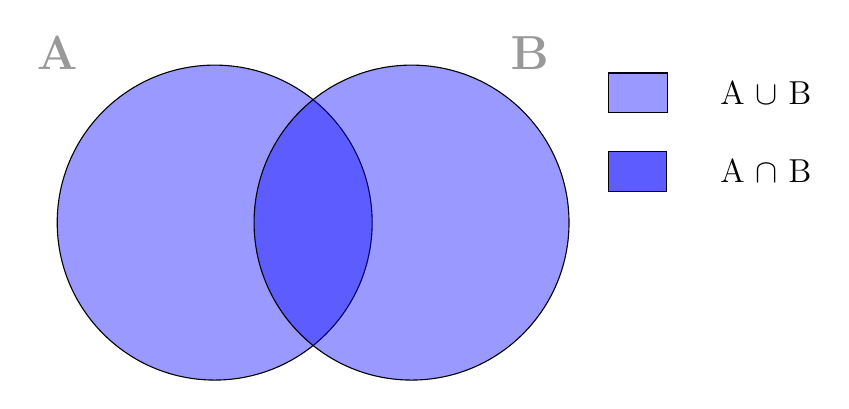
\begin{tikzpicture}

	\begin{scope} [fill opacity = .4]

    \draw[fill=blue, draw = black] (-1,0.85) circle (2);
    \draw[fill=blue, draw = black] (1.5,0.85) circle (2);

    
    \node at (-3,3) {\LARGE\textbf{A}};
    \node at (3,3) {\LARGE\textbf{B}};
    \draw[fill=blue](4, 2.25) rectangle (4.75, 2.75);
    \draw[fill=blue](4, 1.25) rectangle(4.74, 1.75);
    \draw[fill=blue](4, 1.25) rectangle(4.74, 1.75);
    \end{scope}
    \node at (6, 2.5) {\large A $\cup$ B};
    \node at (6, 1.5){\large A $\cap$ B};
\end{tikzpicture}

\end{center}
\begin{framedremark}
    Petite précision à cause du schéma, pour $A \cup B$, tout ce qui est blue est inclus, c'est à dire aussi le bleu foncé.
\end{framedremark}

Pour ce qui est du complément comme dit dans lors de la remarque sur la set universel, le complément de $B$ ressemble à:

\begin{center}
    
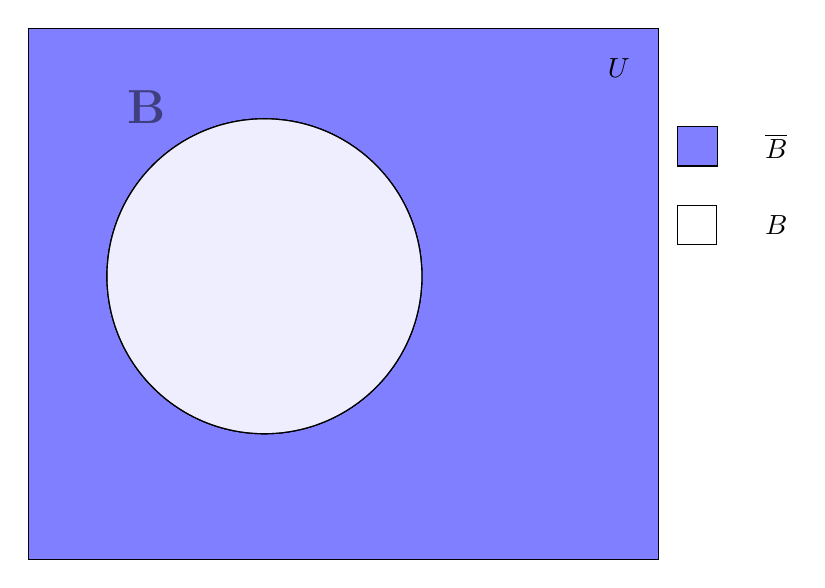
\begin{tikzpicture}

	\begin{scope} [fill opacity = .5]

    

    
    
    
    \draw[fill=blue](4, -2.75) rectangle (-4, 4);
    \draw[fill=white, draw = black] (-1,0.85) circle (2);
    \draw[fill=white, draw = black] (-1,0.85) circle (2);
    \draw[fill=white, draw = black] (-1,0.85) circle (2);

    \draw[fill=blue](4.25, 2.25) rectangle (4.75, 2.75);
    \draw[](4.25, 1.25) rectangle(4.74, 1.75);
    \node at (-2.5,3) {\LARGE\textbf{B}};
 

    \end{scope}
    
    \node at (5.5, 2.5) {$\overline{B}$};
    \node at (3.5, 3.5) {$U$};
    \node at (5.5, 1.5){$B$};
\end{tikzpicture}
\end{center}
On voit ici que $\overline{B} = U - B$.
\\
\hspace{0.4cm}

\noexpand La réflexion durant les exercices est similaires à celle faite pendant les ensembles en analyse. Le but est d'utiliser les définitions des opérations ($\neg$, $\cup$...) afin de comparer différentes relations entre ensembles. 
\\
\begin{exemple}
\\

$A - B$ équivaut à dire : 
\begin{equation*}
    A - B = \{ x | x \in A \wedge x \notin B\}
\end{equation*}
Un autre moyen de l'écrire est :
\begin{equation*}
    A - B = A \cap \overline{B}
\end{equation*}
\end{exemple}
Ce qu'on écrit dans la première relation est : tout les éléments qui sont dans $A$ et qui ne sont pas dans $B$. Dans la deuxième relation, on a l'intersection entre $A$ et le complément de $B$. Pour rappelle, le complément d'un ensemble est la soustraction de l'univers par l'ensemble : $\overline{B} = U - B$. Ce qui veut dire, tout les éléments qui sont dans U (tout les éléments) et qui ne sont pas dans $B$. On sait donc que l'intersection entre ce complément et un autre ensemble ne peut posséder d'éléments se trouvant dans $B$.
\\
L'intersection des ensembles et d'autre opérations sont des analogies de la logique, on y retrouve donc les mêmes opérations comme la loi de Morgan etc... On peut les utiliser pour prouver des équivalences ou montrer si un ensemble est un ensemble vide.
\hspace{0.4cm}
\\
\hspace{0.4cm}
Voici des exemples d'intersection et d'autre opérations logiques appliquées au set: 
\begin{itemize}
    \item $A \cup B = \{x|x \in A \wedge x \in B\}$
    \item $\overline{A} = \{x \in U | x \notin A\} = \{x \in U | \neg( x \in A )\}$
    \item $A \oplus B = \{x|x \in A \oplus x \in B\}$
\end{itemize}
\\
\hspace{0.6cm}
\begin{exemple}
Pour illustrer tout ça, on peut prendre : $(A \cap B) - (A \cap C)$
\begin{align*}
    &= (A \cap B) \cap \overline{A \cap C} \\
    &= (A\cap B) \cap ( \overline{A}\cup \overline{C})\\
    &= (A \cap B \cap \overline{A}) \cup (A\cap B \cap \overline{C})
\end{align*}
On voit qu'ici on a utilisé trois loi dont la première a déjà été énoncée précédemment. On a donc la loi de Morgan afin d'injecter la "\textit{négation}" dans les parenthèse, la loi de Distributivité, afin d'avoir que des intersections dans les parenthèses. A partir de là on peut trouver que $(A \cap B \cap \overline{A}) = \emptyset$ et que donc : 
\begin{equation*}
    (A\cap B ) - ( A \cap C ) = (A \cap B \cap \overline{C})
\end{equation*}
\hspace{0.4cm}
\\
Si on veut maintenant utiliser la logique propositionnel et les "builder" on peut prendre comme exemple l'égalité : 
\begin{equation*}
    \overline{A \cap B} = \overline{A}\cup \overline{B}
\end{equation*}
On voit ici que cela ressemble furieusement (petit ref à Jérome) à la loi de Morgan. En prenant la définition du complément: 
\begin{equation*}
    \overline{A \cap B} = \{X|x \notin (A \cap B)\}
\end{equation*}

Si on rajouter la définition du $\notin$ qui est la négation du $\in$:
\begin{equation*}
    = \{x | \neg(x \in (A \cap B))\}
\end{equation*}
Si on y rajoute l'intersection : 
\begin{equation*}
    = \{x | \neg(x \in A \wedge x \in B)\}
\end{equation*}
Et la fameuse loi de Morgan: 
\begin{equation*}
    =\{ x | \neg(x \in A) \vee \neg(x \in B)\}
\end{equation*}
Et donc si on "\textit{revient}" en arrière avec les définitions du complément et de l'union on à donc:
\begin{equation*}
    = \overline{A} \cup \overline{B}
\end{equation*}
\end{exemple}
qui nous donne l'analogie de la loi de Morgan pour les sets.
\\

\hspace{0.4cm}
Il reste encore deux opérations à énoncer ici qui sont : 
\begin{itemize}
    \item Le cardinal de S : $|S|$ qui est la taille de l'ensemble.
\\
Il existe aussi des identités avec la cardinalité comme $|A \cup B| =|A| + |B| - |A \cap B|$.
    \item Le produit cartésien ( $A \times B \implies$ une set de paires ordonnées ($a$, $b$) où $a \in A$ et $b \in B$). On verra plus tard que ce produit est très utiles notamment pour les relations.)
\end{itemize}
\\
Je vais un peu m'attarder sur le produit cartésien et les Tuples car je trouve ça important par la suite. Donc avant d'introduire le produit cartésien:

\begin{definition}[Tuples]
    Une \textbf{ordered n-tuple} $(a_1, a_2, ..., a_n)$ est une collection ordonnée (donc $(a, b, c) \neq (b, c, a)$) qui possède $a_1$ comme première élément, $a_2$ comme deuxième etc... jusqu'à $a_n$.
\end{definition}
Donc comme dit dans la définition, deux tuples sont égaux si et seulement si chaque élément au même indice sont égaux.
\\
\begin{definition}
    Le \textbf{cartesian product} de deux sets $A$ et $B$, noté $A \times B$, est la set de paires ordonnée $(a, b)$ ou $a \in A$ et $b \in B$. tel que:
\[ A \times B =\{(a, b\}|(a \in A )\wedge (b \in B)\]
\end{definition}
\\
\begin{exemple}
    Si on prend: $A =\{a, b\}$ et $B = \{1, 2, 3\}$:
\[ A \times B =\{(a, 1), (a, 2), (a, 3), (b, 1), (b, 2), (b, 3)\}\] Et dans l'autre sens:
\[ B \times A =\{(1, a), (1, b), (2, a), (2, b), (3, a), (3, b)\}\]
\end{exemple}
Comment on peut le voir est un peu comme un sorte de "\textit{distributivité}" que dans un sens, que c'est chaque élément de la première set avec tout les éléments de l'autre set.
\\
Il est aussi possible de le faire avec plus qu'une set et ça définition est:
\begin{definition}
    Le \textbf{cartesian product} des set $A_1, A_2, ..., A_n$, dénoté par $A_1 \times A_2 \times ... \times A_n$, est la set ordonné d'un tuple de taille $n$ tel que ($a_1$, $a_2$, ..., $a_n$), où les $a_i$ appartiennent à $A_i$ pour $i = 1, ... n$ (comme une boucle \textit{for}).
    \[ A_i \times A_2 \times ... \times A_n  = \{(a_1, a_2, ..., a_n)|a_i \in A_i \; for \; i = 1, 2, ... n\}\]
\end{definition}
J'ai mis for parce que c'est une sorte de boucle qui va se produire à chaque fois pour chaque set. Pour construire le produit de trois set, on va d'abord prendre le première élément des deux première set et faire des tuples avec les éléments de la dernière, ensuite on va prendre le deuxième élément de la première set et faire la même étapes, et dès qu'il y a plus d'élément dans la première set, on recommence mais en changeant l'élément dans la deuxième set. Attention à ne pas se répéter, de ce que j'ai vu la taille du produit cartésien est le produit des tailles des sets.
\paragraph{Predicates avec les sets}
\begin{definition}
    En ayant une predicate $P$ et un domaine $D$, on défini la \textbf{truth set} de $P$ la set des éléments pour laquelle $P(x)$ est vrai.
    \\
    On la note:
    \[\{x \in D| P(x)\}\]
\end{definition}
Je voulais juste mettre ça la pour avoir une définition propre mais normalement ça a déjà été dans les exos.
\\
\subsection{Petit résumé}
On voit ici que pour les sets, les types d'exercices principaux sont : 
\begin{itemize}
    \item Prouver des égalités entre différentes sets
    \item Montrer qu'une set est (ou non) une subset d'une autre set
    \item De la théorie sur les power sets et le cardinal, produit cartésiens...
\end{itemize}
J'ai regardé pas mal d'examen des années précédentes et ce que je vois le plus sont des questions avec quelque set mélangé à des relations ou fonctions mais que relativement rarement un exercice complet sur exclusivement des sets (Il y en a, notamment avec des power set dans l'examen de 2019). 


\section{Fonction}
\begin{definition}[fonction]
    Soit: $A$ et $B$ deux sets non vides. Une fonction $f$ de $A$ à $B$ est une "\textit{assignment}" d'un seul et unique élément de $B$ à chaque élément de $A$.
\end{definition}
\begin{itemize}
    \item Si $f$ va de $A$ à $B$, on note: $f: A \to B$.
\end{itemize}
On peut aussi appeler les fonctions, des \textbf{mappings} ou \textbf{transformation}.
\\
\paragraph{Terminologie}
\begin{itemize}
    \item On dit que $f$ \textbf{maps} de $A$ à $B$
    \item $A$ est appelé le \textbf{domaine} de $f$
    \item $B$ est appelé le \textbf{codomaine} de $f$
    \item Si $f(a) = b$ ,
    \begin{itemize}
        \item alors b est l'image de $a$
        \item $a$ est la préimage de $b$
    \end{itemize}
    \item Deux fonctions sont égales quand elles ont:
    \begin{itemize}
        \item le même domaine
        \item le même codomaine
        \item maps chaque élément du domaines au même élément du codomaine.
    \end{itemize}
\end{itemize}
\begin{center}
    
\begin{tikzpicture}
    \foreach[count=\i] \lseti/\lsetmi in {A/{$a$,$b$,$g$},B/{5,6,$z$}} {
        \begin{scope}[local bounding box=\lseti, x=3cm, y=1cm]
        \foreach[count=\j] \lj in \lsetmi {
            \node[minimum width=2em,anchor=base,text height=1.4ex,text
            depth=0.25ex] (n-\j-\lseti) 
            at (\i,-\j) {\lj};
        }
        \end{scope}
        \node[ellipse, draw, fit=(\lseti), 
        label={[name=l-\lseti]above:$\lseti$}] {};
    }
    \draw[->] (n-1-A) -- (n-1-B);
    \draw[->] (n-2-A) -- (n-2-B);
    \draw[->] (n-3-A) -- (n-3-B);
    \draw[->] (l-A) -- node[above]{$f$}(l-B);
\end{tikzpicture}
\end{center}
\begin{framedremark}
    Attention, des fonctions peuvent avoir la même application mais pas le même domaine donc elle sont pas égales alors qu'elles sont "\textit{pareil}".
\end{framedremark}



\begin{itemize}
    \item On appelle \textbf{Range} de $f$ la set de toute les images de $A$, on l'appelle $f(A)$.
    \item le Range est la set ou il y a que les images, il n'y a pas d'éléments qui ne sont pas images de $f$.
    \item Codomaines vs range pour $f: A \to B$: 
\end{itemize}

\begin{center}
    
\begin{tikzpicture}
    \foreach[count=\i] \lseti/\lsetmi in {A/{$a$,$b$,$g$},B/{5,6,$z$}} {
        \begin{scope}[local bounding box=\lseti, x=3cm, y=1cm]
        \foreach[count=\j] \lj in \lsetmi {
            \node[minimum width=2em,anchor=base,text height=1.4ex,text
            depth=0.25ex] (n-\j-\lseti) 
            at (\i,-\j) {\lj};
        }
        \end{scope}
        \node[ellipse, draw, fit=(\lseti), 
        label={[name=l-\lseti]above:$\lseti$}] {};
    }
    \draw[->] (n-1-A) -- (n-1-B);
    \draw[->] (n-2-A) -- (n-2-B);
    \draw[->] (n-3-A) -- (n-2-B);
    \draw[->] (l-A) -- node[above]{$f$}(l-B);
\end{tikzpicture}
\end{center}
\begin{itemize}
    \item Ici le codomaine est $B$, mais le range est la set : $f(S) = \{ f(S) | s \in S\}$
    \item $f(S) = \{ 5, 6\}$
    \item Attention au majuscule, $f(S)$ est le range contrairement à $f(s)$.
    \item La range est donc une subset du codomaine tq: $f(S) \subseteq B$ où $B$ est le codomaine.
\end{itemize}
\subsection{Surjectif, injectif, bijectif}
Comme se sont des notions qui sont déjà traité en analyse, on va survoler le sujet mais prenons comme exemple la fonction $x^2$: 
\\

\hspace{0.7cm}
\begin{center}
\begin{tikzpicture}[scale=1.5]
\draw[->,line width=1pt] (-2,0)--(2,0) node[right]{$x$};
\draw[->,line width=1pt] (0,-1.5)--(0,2.75) node[above]{$f(x)$};
\draw[blue,line width=1pt,domain=-1.6:1.6, samples=100] plot(\x,{(\x)^2}); % <--- observe parenthesis
\end{tikzpicture}
\end{center}

\begin{definition}[Injectif]
    Un fonction $f$ est dite injective si et seulement si $\forall a\forall b (f(a)  = f(b)) \implies (a = b)$ dans le domaine de $f$
\end{definition}
nous voyons donc que dans $\mathbb{R}$ la fonction $x^2$ n'est pas injective car il est très facile de trouver un contre exemple : 
\begin{equation*}
    f(-1) = f(1)
\end{equation*}
\begin{definition}[surjective]
    Une fonction $f$ est surjective si et seulement si $\forall b \in B \exists a \in A | f(a) = b$ 
\end{definition}
En français, chaque élément du codomaine a une \textit{flèche} qui vient vers lui. Pour notre fonction on voit que par exemple $-1$ qui est un élément de $\mathbb{R}$ n'a pas de préimage. on voit donc que $x^2$ n'est pas surjective.
\\
Afin qu'elle devienne injective, on peut faire en sorte que pour chaque image ($f(x)$), il n'y a qu'un $x$ qui y arrive, pour cela on peut couper le domaine au réel positif.
\\
Afin qu'elle devienne surjective il faut couper à l'endroit où la fonction est toujours définie, on peut prendre donc les réels positif comme codomaine. Pour que $x^2$ soit bijectif on a:
\begin{equation*}
    f: \mathbb{R^+} \to \mathbb{R^+}
\end{equation*}
Ce qui donne sur le graphe:
\begin{center}
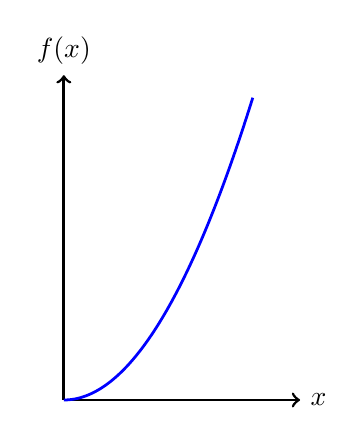
\begin{tikzpicture}[scale=1.5]
\draw[->,line width=1pt] (0,0)--(2,0) node[right]{$x$};
\draw[->,line width=1pt] (0,0)--(0,2.75) node[above]{$f(x)$};
\draw[blue,line width=1pt,domain=0:1.6, samples=100] plot(\x,{(\x)^2}); % <--- observe parenthesis
\end{tikzpicture}
\end{center}
On voit qu'il y a qu'un point pour chaque $f(x)$ et un seul point pour chaque $x$.
\begin{framedremark}
    \textbf{ATTENTION} Dans le quizz de 2022, il y a la question:\\
    une fonction g: \Z $\times$ \Z $\to$ \Z, est-elle surjective?
\[b) \; g(a, b) = 3a + 1\]
\\
La réponse à cette question est non. Pour rappel, la surjectivité d'une fonction est définie par: 
\\
\begin{center}
    Pour tout $b$ dans le codomaine, il existe un $a$ dans le domaine tel que: $f(a) = b$.
\end{center}
Il est très facile de trouver un nombre dans \Z qui n'a pas de "\textit{flèche}" vers lui. On voit que la fonction renvoie tout les multiples de 3 avec une incrémentation de 1. donc il suffit de prendre par exemple $2$ tel que: 
\[f(a, b) = 2\]
Ce qui donne: 
\begin{align*}
    3a + 1 &= 2\\
    3a &= 1 \\
    a &= \frac{1}{3}\\
    a &\notin \mathbb{Z}
\end{align*}
On voit donc que la fonction n'est pas surjective.
\end{framedremark}

\paragraph{Petit résumé}
Le moyen le plus rapide de prouver qu'une fonction n'est pas bijective (ou inj, surj) est le contre exemple. 
\\
Pour prouver qu'elle est bij, inj, surj:
\begin{itemize}
    \item $f$ est injective: montrer que si $f(x) = f(y)$ alors $x = y$
    \item $f$ est surjective: montrer que pour n'importe quelle $y$ du codomaine, il existe un élément $x$ tq $f(x) = y$.
    \item $f$ est bijective si elle a les deux conditions ci-dessus.
\end{itemize}

Quelque info en plus:
\begin{itemize}
    \item si $f$ est une bijection, alors il lui existe un inverse noté à $f^{-1}$.
    \item Rappel qu'il existe les compositions de fonction (comme en analyse)
    \item Une \textbf{fonction partiel} $f$ d'une set $A$ à une set $B$ est un mapping de chaque élément $a$ d'une subset $S$ où $S \subseteq A$, appelé le domaine de définition de $f$, à un unique élément $b$ dans $B$.
    
\end{itemize}




\section{Relations}

\begin{definition}[Binary Relations]
    Une \textbf{binary relation} $R$ depuis une set $A$ jusqu'à une set $B$ est une subset: $R \subseteq A \times B$.
\end{definition}
\\
En français, une relation est un façon de relier des éléments de $A$ avec des éléments de $B$ (en pair). On sait aussi que $R$ est une subset du produit cartésien, ce qui signifie qu'il peut y avoir toute les pairs possibles. Prenons un exemple des slides:
\\
Soit $A = \{0, 1, 2\}$ et $B = \{a, b\}$, alors:
\begin{itemize}
    \item $A \times B = \{(0, a), (0, b), (1, a), (1, b), (2, a), (2, b)\}$
    \item $R_1 = \{(0, a), (0, b)\}$ est une relation de $A$ à $B$.
\end{itemize}

Essayons de visualiser avec des un graphe dirigé (avec des flèches):
\begin{center}
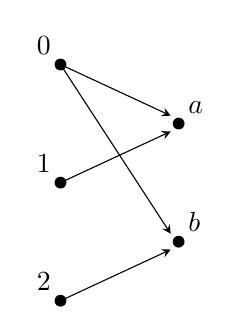
\begin{tikzpicture}
    \fill[black](0, 0) circle (0.075) node[above left]{$0$};
    \fill[black](0, -1.5) circle(0.075) node[above left]{1};
    \fill[black](0, -3) circle(0.075) node[above left]{2};
    \fill[black](1.5,-0.75) circle(0.075) node[above right]{$a$};
    \fill[black](1.5, -2.25) circle(0.075) node[above right]{$b$};

    \draw[-stealth](0, 0) -- (1.4, -0.65);
    \draw[-stealth](0, -1.5) -- (1.4, -0.85);
    \draw[-stealth](0, 0) -- (1.4, -2.15);
    \draw[-stealth](0, -3) -- (1.4, -2.35);

    
\end{tikzpicture}
\end{center}
\\

On voit que les relations sont de $0$ à $a$ , 1 à $a$, 2 à $b$ et $1$ à $a$. ce qui donne comme relation:
\[ R =\{(0, a), (1, a), (0, b), (2, b)\}\]
On voit donc qu'il y a quand même une différence entre fonction et relation, par la définition des fonctions la relation présenté ci-dessus ne peut pas être représenté comme une fonction.

\paragraph{Fonction et relation}
\begin{itemize}
    \item On voit qu'une fonction: $f : A \to B$ peut aussi être défini par une subset de $A \times B$ aka une relation.
    \item Une fonction $f$ de $A$ à $B$ contient une et uniquement une pair (a, b) (ordonnée) pour chaque $a \in A$.
\end{itemize}
En gros les relations sont plus général que les fonctions et elles les englobent. c'est pour cela qu'une relation ne peut pas toujours s'écrire comme une fonction.
\begin{itemize}
    \item Soit $A = \{a, b, c\}$
    \item Alors $R = \{(a, a), (a, b)\}$ est une relation sur $A$.
    \item Soit $A= \{1, 2, 3, 4\}$
    \item Alors $R = \{(a, b) | a < b\}$ est une relation sur $A$.
\end{itemize}

La dernière relation signifie en français: toute les paires de nombres ou $a$ est plus petit que $b$. on y retrouve par exemple la pair : $(1, 2)$.

\begin{definition}[Reflexive]
    Une relation $R$ sur une set $A$ est \textbf{reflexive} si et seulement si $(a, a) \in R$ pour tout $a \in A$.
\end{definition}
Pour chaque élément, il y a la pair avec lui même, Par exemple: 
\begin{equation*}
    S =  \{ 1, 2, 3, 4\}
\end{equation*}
On voit ici que pour qu'une relation $R$ soit reflexive alors Il faut qu'il y ait les relations : 
\begin{equation*}
    R = \{(1, 1), (2, 2), (3, 3), (4, 4)\}
\end{equation*}
\hspace{0.4cm}

\begin{definition}[Symmetric]
    Une relation $R$ sur une set $A$ est \textbf{symmetric} si et seulement si $(b, a) \in R$ à chaque fois que $(a, b) \in R$ pour tout $a, b \in A$.
\end{definition}
Par exemple, si on prend une relation symmetric, ça donne:
\begin{equation*}
    R = \{(1, 2), (2, 3), (2, 1), (3, 2)\}
\end{equation*}
Pour chaque paires d'éléments, il y a la paire "\textit{inverse}".

\begin{definition}[Antisymmetric]
    Une relation $R$ sur une set $A$ est \textbf{antisymmetric} si et seulement si, quand $(a, b) \in R$ et $(b, a) \in R$ alors $a = b$ pour tout $a, b \in A$
\end{definition}
Ce qui veut dire que si il y a un symmetric, c'est forcémment une reflexion sinon ce n'est pas une relation antisymmetric. En image ça donne: 
\begin{equation*}
    R = \{ (1, 1), (2, 2), (3, 4)\}
\end{equation*}
On voit ici que la suite est antisymmetric mais pas reflexive. elle le serait sans la paire $(3, 4)$. La paires $(3, 4)$ n'enlève pas la propriété antisymmetric car on ne trouve pas dans la suite l'"\textit{inverse}" $(4, 3)$. 
\\
\textbf{Attention} antisymmetric n'est pas l'opposée de symmetric.


\begin{definition}[Transitive]
    Une relation R sur une set $A$ est appelée \textbf{transitive} si et seulement si lorsque $(a, b) \in R$ et $(b, c) \in R$ alors, $(a, c) \in R$ pour tout $a, b, c \in A$.
\end{definition}
C'est comme une composition de fonction, ou une addition de vecteur en géométrie :


\begin{center}
    
\begin{tikzpicture}[line cap=round]
  \coordinate (O) at (0,0);
  \coordinate (A) at ( -3:2.1);
  \coordinate (B) at ( 55:1.4);
  \coordinate (A+B) at ($(A)+(B)$);
  
  \draw[vector, arrow,myred] (B) -- (A+B) node[midway,above] {$\vb{(b, c)}$}; 
  
  \draw[vector,myblue] (O) -- (B) node[midway,above left] {$\vb{(a,b)}$};
  \draw[vector,mypurple] (O) -- (A+B) node[above right=-1.5] {$\vb{(a},\vb{c)}$};
\end{tikzpicture}
\end{center}
\\
On a ici l'illustration en géométrie de la propriété de transitivité des relations.


\begin{definition}[Equivalence Relations]
    Une relation sur une set $A$ est appelée \textbf{equivalence relation} si et seulement si elle est reflexice, symmetric et transitive.
\end{definition}


\paragraph{Nombre de relation}
Nombre de relation pour une set $A$ avec $|A|$ éléments:
\begin{itemize}
    \item $A \times A$ possède $|A|^2$ éléments (pour $|A|$ élément dans $A$)
    \item Toute les subset de $A \times A$ peut être une relation
    \item Donc, il y a $2^{|A|^2}$ relations possibles dans une set $A$.
\end{itemize}
On trouve ce résultat grâce à la power set qui nous dit que pour tout set de taille $n$ il existe $2^n$ subset.

\begin{definition}[Equivalence Classes]
    Soit $R$ une relation d'équivalence sur une set $A$. La set de tout les éléments qui sont relié à un élément $a$ de $A$ a
\end{definition}
Imaginons que tu as un ensemble $A$ de plusieurs éléments (par exemple, des nombres, des personnes, ou n'importe quoi). Une relation d'équivalence R est une façon de dire quels éléments de $A$ sont "liés" entre eux d'une manière qui respecte les trois propriétés d'équivalence.
\\
\begin{exemple}
    
Soit une set $A = \{1, 2, 3, 4, 5, 6\}$ et la relation $R = \{(a, b) \in A|$ $a$ et $b$ sont congru modulo 2 (même reste)$\}$.
\begin{itemize}
    \item Alors les nombres, $2, 4, 6$ sont tous lieés entre eux parce qu'ils sont tous pairs. $[2] = \{2, 4, 6\}$
    \item Et les nombres $1, 3, 5$ sont aussi liées entre eux parce qu'ils sont tous impairs. $[1] = \{1, 3, 5\}$
\end{itemize}
Il y donc deux classe d'équivalences : 
\begin{itemize}
    \item la classe de 2 (qui a tout les nombres pairs):  $[2] = \{2, 4, 6\}$.
    \item la classe de 1 (qui a tout les nombres impairs):   $[1] = \{1, 3, 5\}$.
\end{itemize}
La classe d'équivalence d'un élément $a$ (notée [a]) est simplement l'\textbf{ensemble de tous les objets de A qui sont liés à }$a$ par la relation d'équivalence. Dans l'exemple, [2] regroupe tous les nombres pairs, car ils sont tous "équivalents" sous cette relation.
\end{exemple}

\begin{framedate}
   Cours: 09/10/2024
\end{framedate}

\section{Partition of a Set}
\begin{definition}[Partition]
    Une \textbf{partition} d'une set $S$ est une collection de \textit{disjonction de sub sets non-vides} de $S$ qui ont $S$ comme union.
\end{definition}
La collection de subsets $A_i$, où $i \in I$ forme une partiotion de $S$ iff (si et seulement si) :
\begin{itemize}

    \item $A_i = \emptyset for i \in I$ \vspace{0.4cm} Subsets non vide
    \item $A_i \cap A_j = \emptyset$ when $i \noteq  j $ \vspace{0.2cm} disjoint des subsets (tout les sets n'ont aucun point commun)
    \item \[\bigcup_{i\in I}^n A_i = S \] Ce qui équivaut à que tout les subsets $A_i$ ensemble regroupe $S$ (l'union est $S$).
\end{itemize}
En français il y a trois critère:
\begin{itemize}
    \item Les subsets sont non vides
    \item Les subsets n'ont aucun éléments en commun.
    \item L'union de toute les subsets forme $S$.

\end{itemize}
Donc cela veut dire qu'il faut toute les subsets afin de créer la set $S$. 
\begin{framedremark}
    Cela ne veut pas dire que les subsets $A_i$ sont tout de même taille. une pourrait avoir la plupart des éléments voir tous.
\end{framedremark}

\hspace{0.4cm}

\begin{definition}[Partial Ordering]
    Une relation $R$ sur une set $S$ est appelée \textbf{partial ordering}, ou partial order, si elle est \textit{reflexive, antisymmetric} et \textit{transitive}.
\end{definition}
\\
\begin{framedremark}
    Le "\textit{type}" d'une partial ordering est une \textbf{relation} (ne pas comfondre avec la \textit{partition} d'une set).
    \end{framedremark}
    
Une set avec un partial ordering R est appellé une partially ordered set, ou \textbf{poset}, et elle est notée par $(S, R)$.
\\
C'est peut-être pas très clair vu comme ça, donc regardons avec un 

\begin{exemple}
    

Soit $R = \{(a, b) \in \mathbb{Z} \times \mathbb{Z}| a \geq b\}$.
\\
On voit ici que:
\begin{itemize}
    \item $R$ est reflexive grâce au $\geq$ qui nous donne le $=$ avec car $a \geq a$, donc $(a, a) \in R$.
    \item $R$ est antisymmetric car si $a \geq b \wedge b \geq a$ alors forcémment $a = b$ (ce qui est à quelque mots près, la définition d'antisymmetric).
    \item $R$ est logiquement transitive, car si $a \geq b$ et que $b \geq c$ alors forcémment $a \geq c$.
\end{itemize}
\\

On a donc que $R$ est une partial ordering sur $\mathbb{Z}$ et ($\mathbb{Z}, \geq$) est une \textbf{poset}.

\end{exemple}

\begin{framedremark}{Notation}
    Différentes posets utilisent donc différents symboles (i.e $\geq$ vu précédemment), Pour noter une relation arbitraire on utilise le symbole: $\preceq$ ($\preceq$ signifie donc une relation arbitraire qui pourrait être n'importe quoi ($a$ divise $b$ par exemple)).
\end{framedremark}
\\

\begin{exemple}
Est ce que la relation $|$ (divides) est une partial ordering on $\mathbb{Z}^+$?
\begin{itemize}
    \item \textbf{reflexive}: car $a | a$ pour tout $a \in \mathbb{Z}^+$
    \item \textbf{antisymmetric}: grâce à la définition d'au dessus, si $a | b$ et que $b | a$ alors la seule possibilité est: $a = b$
    \item \textbf{transitive}: Si on prend la définition : $a \preceq b \wedge b \preceq c$ et qu'on la traduit en français :
\\
\textit{si $a$ divise $b$ et que $b$ divise $c$, alors $a$ divise $c$}, On peut prendre que, $a\cdot n = b$ et $b * m = c$. on peut écrit que $a\cdot n = \frac{c}{m}$. Si on multiplie par $m$, $a\cdot n \cdot m = c$. On voit bien ici que a divise donc m.

\end{itemize}
\end{exemple}



\paragraph{Comparabilité}
\begin{definition}[Comparabilité]
    Les éléments $a$ et $b$ d'une poset ($S, \preceq)$ sont \textbf{comparable} si $a \preceq b$ ou $b \preceq a$. Quand $a$ et $b$ sont des éléments de $S$ tel que ni $a \preceq b$ ni $b \preceq a$ alors, on note que $a$ et $b$ sont \textbf{incomparable}.
\end{definition}
\begin{framedremark}
    Quand $a$ et $b$ sont des éléments d'une poset $(S, \preceq)$, il n'est pas obligatoire que $a \preceq b$ ou $b \preceq a$ et vis-versa. c'est comme symmetric et antisymmetric, c'est pas noir ou blanc, il y a aussi du gris. Il existe des poset où il y a des $a$ et $b$ comparable et d'autre élément $(f, l)$ qui sont incomparable.
\end{framedremark}
\begin{exemple}

Pas tout les éléments d'une poset sont comparable, si on prend l'exemple précédent avec la poset: $(\mathbb{Z}^+, |)$ alors on peut prendre $7$ et $9$, on voit que ces deux éléments sont \textbf{incomparable}.
\end{exemple}
\\

\begin{definition}
    Si $(S, \preceq)$ est une proset et que pour tout deux éléments de $S$, ils sont comparable, S est notée \textbf{totally ordered} ou \textbf{lineary ordered} set, et $\preceq$ est noté \textbf{total order} ou \textbf{linear order}.
\end{definition}
\\
\begin{exemple}
\begin{itemize}
    \item La poset $(\mathbb{Z}, \geq)$ est totally ordered.
    \item La poset $(\mathbb{Z}^+, |)$ n'est \textbf{pas} totally ordered
\end{itemize}
En gros, pour toute paires d'éléments $a$ et $b$, il faut soit $a \preceq b$, soit $b \preceq a$. C'est pour cela que $(\mathbb{Z}^+, |)$ n'est pas totally ordered (7 et 9 par exemple).
\\
On peut facilement démontrer qu'une poset n'est pas totally ordered en trouvant un contre exemple.
\end{exemple}
\\
\begin{definition}
    $(S,\preceq)$ est une \textbf{well-ordoered} set si elle est une poset tel que $\preceq$ est un \textit{total ordering} et que toute les subsets non-vides de $S$ possède un \textit{least} élément.
\end{definition}

\begin{exemple}
\\

Soit la poset $(\mathbb{Z}^+, \leq$): Alors elle est \textit{well-ordered}. La raison et que pour n'importe quelle subset qu'on prends, on peut toujours trouver le \textit{least element} qui est le plus petit.
\\
Si on faisait des relations, le \textit{least element} se trouve toujours du côté gauche de la paire. voici un moyen de se le visualiser.
\\
Si on prenait la poset: ($\mathbb{Z}, \geq$), on voit que la poset n'est pas \textit{well ordered} comme on à tout l'ensemble $\mathbb{Z}$ on peut toujours aller soit à l'infini sur la gauche ou l'infini sur la droite.
\end{exemple}
\begin{framedremark}
    Attention ici c'est le plus petit mais c'est pas toujours le plus petit
\end{framedremark}

\subsection{Hasse Diagrams}
Represente une \textbf{poset} avec un graphe:
\begin{itemize}
    \item Les nodes sont des éléments de la set
    \item Les \textbf{edges} connectent les éléments qui ont une relation
    \item Les self-relations ne sont pas représenté
    \item les relations transitive ne sont pas representé (elles sont implicites):
    \begin{itemize}
        \item si $a \preceq b$ et que $b \preceq c$ alors on sait que $a \preceq c$.
        \item Par raison de clarité, aucun chemin sera entre $a$ et $c$
    \end{itemize}
    \item Les chemins n'ont pas de direction, on assume qu'elle vont vers le haut.
\end{itemize}
\\

Considérons la poset ($\{1, 2, 3, 4\}, \leq$). On peut en 1), enlever les self-loop (ceux qui part et vont sur eux-même), 2) enlever les chemins transitifs (comme vu avec les vecteurs) et en 3) assumer que les pointes des flèches vont toujours vers le haut.
\\
\begin{exemple}
On peut se visualiser le hasse diagrams de la power set de $\{a, b\}$ :
\\
\begin{center}
\begin{tikzpicture}
    \matrix (A) [matrix of nodes, row sep=1.2cm]
    { 
        & $\{a,b\}$ \\  
	$\{a\}$ &  & $\{b\}$\\
        & $\emptyset$ \\
    };
    \draw (A-1-2)--(A-2-1);
    \draw (A-1-2)--(A-2-3);
    \draw (A-2-1)--(A-3-2);
    \draw (A-2-3)--(A-3-2);
\end{tikzpicture}
\end{center}
On voit ici que le diagram est assez "\textit{simple}", mais il peut très vite tourner au cauchemar, Si on prends juste la power set de $\{a, b, c\}$ le diagram donne:
\begin{center}
\begin{tikzpicture}
    \matrix (A) [matrix of nodes, row sep=1.2cm]
    {
        $\{a,b\}$ & $\{a,c\}$ & $\{b,c\}$ \\
        $\{a\}$ & $\{b\}$ & $\{c\}$ \\
        & $\emptyset$ \\
    };
    \path (A-1-1)--(A-1-2) node[above=1.2cm] (link) {$\{a,b,c\}$};
    
    \foreach \i in {1,...,3}
    \draw (link.south) -- (A-1-\i.north);
    \foreach \i/\j in {1/2, 3/2, 2/1, 1/1, 3/3, 2/3}
    \draw (A-1-\i.south)--(A-2-\j.north);
    \foreach \i/\j in {1/2, 2/2, 3/2}
    \draw (A-2-\i.south)--(A-3-\j.north);
\end{tikzpicture}
\end{center}
Je vous donne le lien du site où il y a $\{a, b, c, d\}$.
\\
On voit donc que $\emptyset$ est toujours dans les powersets. Si on veut trouvers la powerset de $\{a, b\}$, on doit donc redescendre (les flèches vont que vers le haut). On a donc que dans la superset de $\{a, b\}$ il y a $\{a\}$ et $\{b\}$ et aussi $\emptyset$  (et $\{a, b\}$).

\end{exemple}



\paragraph{Partial Order on Cartesian Product}
\begin{definition}[lexicographic ordering]
Soit deux posets $(A_1, \preceq_1)$ et $(A_2, \preceq_2)$ le \textbf{lexicographic ordering} sur $A_1 \times A_2$ est définie en spécifiant que $(a_1, a_2)$ est moins que ($b_1, b_2$), ce qu'est:
$(a_1, a_2) \prec (b1, b2)$, 
soit $a_1 \prec_1 b_1$ ou (si $a_1 = b_1$ et $a_2 \prec_2 b_2)$.
\end{definition}
\\

On peut aussi l'appeler \textbf{dictionary order}.

\begin{exemple}
    
Prenons $(\mathbb{Z}^+, \leq)$ et $(\mathbb{Z}^+, \leq)$, alors:
\begin{equation*}
    (\mathbb{Z}^+ \times \mathbb{Z}^+, \prec) 
\end{equation*}

On peut prendre comme autre exemple, comment on range les étudiants en IC à partir de leur nom de famille. La première \textit{colonne} serait seulement la première lettre, ensuite on mettrait pour la deuxième colonne la deuxième lettre... Le principe est qu'au lieu d'avoir un ranking en "\textit{1d}" on utilise d'autre "\textit{critère}" (par exemple la deuxième et troisième lettres) afin de classer les éléments.

\end{exemple}

\begin{resume}
\\
    \begin{itemize}
        \item Une relation est la généralisation d'une fonction
        \item Une poset est la généralisation de l'inégalité
    \end{itemize}
\end{resume}

\section{Sequences}
\begin{definition}[sequence]
    Une \textbf{sequence} (suite en fr) est une fonction depuis une subset d'entier (généralement $\{0, 1, 2, ...\}$ ou $\{1, 2, 3, ...\}$) à une set $S$.
\end{definition}
\paragraph{Notation}
Soit $f : \mathbb{N} \to S$ la fonction qui définit la sequence.
\begin{itemize}
    \item On appelle $a_n$ l'image $f(n)$ de l'entier $n$.
    \item On appelle $a_n$ un terme de la sequence.
    \item on appelle la sequence dans son entierté par $\{a_n\}$
\end{itemize}
\begin{framedremark}
    On voit ici que la définition est la même que celle de la suite vu en analyse.
\end{framedremark}

\paragraph{Arithmetic Progression/Geometric Progression}
\begin{definition}[arithmetic progression]
    Une \textbf{arithmetic progression} est une sequence de la forme:
    \[a, a+d, a+2d, ..., a+nd\]
\end{definition}
Où le \textbf{initial term} $a$ et la \textbf{common difference} $d$ sont des nombres réels. Une arithmetic progression est dlfinie par la fonction:
\begin{equation*}
    f:\mathbb{N} \to S, f(n) = a + nd
\end{equation*}
\begin{framedremark}
    on voit ici presque la même définition que la suite arithmétique en analyse avec la raison $r$ qui est l'analogie du $d$.
\end{framedremark}


\begin{definition}[geometric progression]
    Une \textbf{geometric progression} est une sequence de la forme :
\[a, ar, ar^2, ar^3, ..., ar^n\]
\end{definition}
Où le \textbf{inital term} $a$ et le \textbf{common ratio} $r$ sont des nombres réels. Une geometric progression est dfinie par la fonction:
\begin{equation*}
    f:\mathbb{N} \to S, f(n) = ar^n
\end{equation*}

\paragraph{Strings}
\begin{definition}
    Une \textbf{string} est une sequence finie de caractère (chars) depuis une set $A$ finie (l'alphabet)
\end{definition}
\\
Une \textit{string} est définie par la fonction: $:\{0, 1, ..., n\} \to A$
\\
La \textit{empty string} est notée $\lambda$.
\begin{framedremark}
    Les sequences de chars ou bits sont très important en CS.
\end{framedremark}

\paragraph{Recurrence Relations}
\begin{definition}
    A \textbf{recurrence relation} pour une sequence $\{a_n\}$ est une équation qui met $a_n$ en relatio avec un/ou plusieurs terme précédent.
\end{definition}
\\

La \textbf{initial conditions} d'une sequence définit les terms $a_0, a_1, a_2, ...a_{k-1}$.
\\
\begin{exemple}

Soit $(\{)a_n)$ une sequence qui satisfait la relation de réccurrence $a_n = 3a_{n-1}$ pour $n=1, 2, 3, ..$, on suppose que $a_0 = 1$.
\\
Trouver une formule tel que $a_n = adnak$, depuis la relation de récurrence s'appelle: \textbf{solving recurrence relation}.
\\
Cette formule est notée \textbf{closed formula}.
\\
Le but avec ça est de trouver un "\textit{pattern}" en allant, soit en avant (en partant de $a_0$ jusqu'à "\textit{deviner $a_n$}") ou en allant en arrière, en partant de la relation de récurrence en remplaçant $a_{n-1}$ par sa relation précédente comme avec des poupées russes.
\\
Si on prend $a_n = a_{n-1} + 3$ et qu'on va en arrière on a:
\begin{align*}
    a_n &= a_{n-1} + 3 \\
    &= (a_{n-2}+3)+ 3 \\
    &= (a_{n-3}+ 3) + 3 + 3
\end{align*}
A partir de là, on peut assumer que c'est une sequence arithmetic avec une progression de $3$.
\end{exemple}
